\mysection{Realization}
In general, this chapter describes the methodical procedure of solving the problem mentioned in \subsecref{Terms of Referencee}. After describing the used dataset all required software and hardware components are explained in detail. Furthermore, the chapter leads through the installation steps of Tensorflow and the setup of Android Studio. Followed by the installation process the retraining of a pre-trained model is depicted. Afterwards, the re-trained model is tested and validated. The chapter ends with the description of the realization of the Android app.

	\mysubsection{Dataset}
The most famous image dataset is ImageNet which is known from the ILSVRC2012. It contains overall about 14 million Images \citep{ImageNet2010}. This dataset is also used for nearly all pre-trained models. The dataset includes a set of 120 different dog breeds with about 150 images each breed. This dog dataset can be downloaded from the following Stanford website \url{http://vision.stanford.edu/aditya86/ImageNetDogs/}. \\
Another dataset with dogs is from Udacity and can be downloaded from \url{https://s3-us-west-1.amazonaws.com/udacity-aind/dog-project/dogImages.zip}. It contains 133 dog breeds with a mean of 63 images each breed. The images in this dataset are completely different from the ImageNet dataset. \\

Because of the reason that the ImageNet dataset is already used to train the pretrained models, the last dataset is used for this project, which is fully unknown for any pretrained model.

	\mysubsection{Hardware environment}
Different hardware setups are used for this project to compare the performance of the mobile application.
At first the lowest one is a notebook with an Intel(R) Core(TM) i7-4720HQ CPU @ 2.60GHz and 16GB memory.
The other one is a powerful desktop computer with an Intel(R) Core(TM) i7-6700K CPU @ 4.4 GHz and 16 GB memory.
In this computer there is also a NVIDIA GeForce GTX 980 with CUDA capabilities version 5.2. It has 2048 CUDA cores running @ 1.291 GHz and 4 GB memory.

For good performance comparison of the mobile application also two different mobile phones are used. The first one is a Samsung Galaxy S4 (GT-I9515) with a Qualcomm Snapdragon S600 Quad-Core @1.9 GHz (32-bit) and 2 GB memory. The operating system is Android 5.0.1 (API 21) is running.
The other one is a Motorola Moto X (2nd Gen, 2014) with a Qualcomm Snapdragon 801 Quad-Core @2.5 GHz (32-bit, ARMv7-ISA) and 2 GB memory. Here, the operating system is Android 6.0 (API 23).

	\mysubsection{Installation of software} 
This chapter describes all necessary steps for installing the software environment including Tensorflow.

 			\mysubsubsection{Prerequisites}
The software environment was set up on the Linux distribution Ubuntu 16.04 LTS. To install the software environment for Tensorflow, Python is required. Therefore, the current version of Python 3.6 was installed by default. Tensorflow also supports Bazel which was installed by following command.

\begin{lstlisting}[caption=Bazel Installation, label=list:bazel, language=bash]
	sudo apt-get install openjdk-8-jdk
	
	echo "deb [arch=amd64] http://storage.googleapis.com/bazel-apt stable jdk1.8" | sudo tee /etc/apt/				sources.list.d/bazel.list
	curl https://bazel.build/bazel-release.pub.gpg | sudo apt-key add -
	
	sudo apt-get update && sudo apt-get install bazel
	
	sudo apt-get upgrade bazel
\end{lstlisting}	

Futhermore, the package and environment management tool Anaconda was installed by the following steps:
First, the Anaconda installer was downloaded from \url{https://www.anaconda.com/download/#linux}. During the installation process the prompts were answered by the default suggestions except the following prompt: "Do you wish the installer to prepend the Anaconda3 install location to PATH in your /home/aw/.bashrc ? [yes|no]". "yes" was typed in and conda was tested using the "conda list" command. \\

In the development of native Android Apps, Java is used as the programming language. Within the installation of Anaconda, the JDK in the version 8 was installed.

 	- CUDA, CUDNN
 	
			\mysubsubsection{Tensorflow based on Python}
First, there are some necessary dependencies to install before the actual installation can begin (refer to \listref{python_dependencies}).
\begin{lstlisting}[caption=Installing the dependecies for Tensorflow based on Python 3.n, label=list:python_dependencies, language=bash]
	sudo apt-get install python3-numpy python3-dev python3-pip python3-wheel
\end{lstlisting}

In order to install Tensorflow with Anaconda, an Anaconda environment must be created using following command (refer to \listref{tensorflow_anaconda}).

\begin{lstlisting}[caption=Creating an Anaconda environment, label=list:tensorflow_anaconda, language=bash]
	conda create -n tensorflow python=3.6
\end{lstlisting}

This command depends on the version of Python installed on the computer. Next, the created environment is activated through following line (\listref{activation_anaconda}).

\begin{lstlisting}[caption=Activating the Anaconda environment, label=list:activation_anaconda, language=bash]
	source activate tensorflow
\end{lstlisting}

Futhermore, Tensorflow was installed through the Anaconda environment for CPU only by the following command (refer to \listref{installing_tensorflow_anaconda}).

\begin{lstlisting}[caption=Installing Tensorflow through Anaconda, label=list:installing_tensorflow_anaconda, language=bash]
	pip install --ignore-installed --upgrade https://storage.googleapis.com/tensorflow/linux/cpu/	tensorflow-1.4.1-cp36-cp36m-linux_x86_64.whl
\end{lstlisting}

For GPU the tfBinaryURL was changed to \url{https://storage.googleapis.com/tensorflow/linux/gpu/tensorflow_gpu-1.4.1-cp36-cp36m-linux_x86_64.whl}. \\

In order to validate the installation, a following short Python script was executed in the Anaconda environment (refer to \listref{validation_installation}).

\begin{lstlisting}[caption=Installing Tensorflow through Anaconda, label=list:validation_installation, language=python]
	# Python
	import tensorflow as tf
	hello = tf.constant('Hello, TensorFlow!')
	sess = tf.Session()
	print(sess.run(hello))
\end{lstlisting}

If the output is 'Hello, TensorFlow!', the installation was conducted sucessfully. Each time when working with Tensorflow, the environment has to be activated using the command in \listref{activation_anaconda}. As a consequence, the environment has to be deactivated when the work is done using the command 'deactivate'.

			\mysubsubsection{Tensorflow based on Bazel}
Another way of working with Tensorflow is using Bazel. In order to install, refer to \listref{bazel}. 
After the Bazel installation is completed, the Tensorflow repository can be cloned by following command (refer to \listref{clone_tensorflow}).

\begin{lstlisting}[caption=Cloning the tensorflow repository, label=list:clone_tensorflow, language=bash]
	git clone https://github.com/tensorflow/tensorflow		
\end{lstlisting}

Now, the installation can be configured. The configuration and its prompts are shown in \subsecref{Configure Bazel for Tensorflow}. If GPU usage is desired, some configurations might differ from the shown configuration steps. The differences are explained in \subsubsecref{Prerequisites}.\\

Furthermore, the Android SDK and NDK must be added to the workspace of Bazel. This is done by removing the comments in the WORKSPACE file which is located in the source directory of the Tensorflow repository and adapting the PATH variable according to the location of the SDK and NDK. NDK 16 which was released on November 2017 is incompatible with Bazel. \\

Then, the Tensorflow pip package can be built by Bazel using the command shown in \listref{pip_package} which also enables Streaming SIMD Extensions 2 introduced by Intel Corporation to process data with doubled accuracy. For GPU support the option '--config=cuda' was added to the build command.

\begin{lstlisting}[caption=Building the Tensorflow pip package, label=list:pip_package, language=bash]
	bazel build -c opt --copt=-msse4.2 //tensorflow/tools/pip_package:build_pip_package
	bazel-bin/tensorflow/tools/pip_package/build_pip_package /tmp/tensorflow_pkg
\end{lstlisting}

Finally, the pip package is installed by executing the following command \listref{pip_install}.

\begin{lstlisting}[caption=Installing the pip package, label=list:pip_install, language=bash]
	sudo pip install --upgrade /tmp/tensorflow_pkg/tensorflow-*.whl
\end{lstlisting}

Instead of using the placeholder '-*', the version can also be specified. Which Tensorflow version is used, can be determined by executing 'pip list \big \vert grep tensorflow' depending on the Python version. The version of Tensorflow used in this work is 1.4.1. The validation of the installation is done by executing the command shown in \listref{validation_installation}.

			\mysubsubsection{Installing Android Studio and its Delevopment Kit}
As an app development environment the free IDE Android Studio in its version 3.0.1 was installed by downloading from \url{https://developer.android.com/studio/index.html}. After the archive file was extracted, the script studio.sh was executed. Required dependencies are installed by Android Studio itself. Futhermore, Android Studio automatically installs the necessary SDK and NDK. So, the SDK in the version 26.1.1 and the NDK in its version 16.1 were used. If Android Studio doesn't install the necessary Development Kits, the appropriate SDK and NDK version can be installed by selecting the SDK and NDK in the section File - Settings - Appearance and Behaviour - System Settings - Android SDK. Thereby, in order to avoid any collapses when running the app, it's important to check the used Tensorflow version in the dependency which has to correspond to the Tensorflow version which was used to retrain the model.\\





		\mysubsection{Building the models}
In this section the build and train respectively retrain process are described. At the end a short comparison of execution time on the different hardware setup specified in \subsecref{Hardware environment} is done.
			\mysubsubsection{Execution methods}
After setting up the hole software environment whether with python or bazel or with GPU support or without, the models can be trained. For several reasons as already explained in \subsecref{Key requirements for an appropriate dataset} and \subsecref{Dataset} pretrained models are used for this project. So the next step now is to download such a pretrained model and retraining it. Certainly with the script used for retraining the desired pretrained model will be already downloaded automatically. \\

Generally on retraining all existing weights of the pretrained model will be leaved untouched except for the final layer which is retrained from scratch. Thus, the pretrained model with its primal tasks or labels is adapted to new labels respectively restricted to certain labels or even adapted to new tasks. This technique is also called transfer learning. \citep{TensorFlowRetrain2017}

For easier use some variables has been defined which are shown in \listref{variables}. Some of them must be changed depending on the used model, others are optionally. All these variables are used in the entire project for every execution of a python script or an executable built by bazel!

\begin{minipage}{\linewidth}
\begin{lstlisting}[caption=Defining terminal variables, label=list:variables, language=bash]
	#for InceptionV3 models	use:
	INPUT_SIZE=299					#size of input layer
	ARCHITECTURE=inception_v3	#name of architecture
	INPUT_LAYER=Mul				#name of input layer
	#OUTPUT_LAYER=softmax		#name of output layer (only pretrained model)
	OUTPUT_LAYER=final_result	#name of output layer (after retraining)
	
	#for MobileNet models use:
	INPUT_SIZE=224					#size of input layer
	VERSION=0.50					#version of MobileNet
	ARCHITECTURE=mobilenet_${VERSION}_${INPUT_SIZE}	#name of architecture
	INPUT_LAYER=input	 			#name of input layer
	#OUTPUT_LAYER=MobilenetV1/Predictions/Reshape_1	#name of output layer (only pretrained model)
	OUTPUT_LAYER=final_result	#name of output layer (after retraining)
	
	#optional
	DOG_PATH=${HOME}/dog_photos	#path with images for retraining
	RETRAIN_PATH=${HOME}/MobileInceptionRetrained	#path for all output data
	TRAINING_STEPS=500			#how many training steps
	LEARNING_RATE=0.01			#learning rate
\end{lstlisting}
\end{minipage}

To retrain the model the python script \textit{code/scripts/retrain.py} in the github-repo of this project is used and executed as shown in \listref{retrain}. This script is taken from the 'tensorflow-for-poets'-tutorial and is extended with some time measurings. All important parameters are in the listing mentioned before and explained later in this section. However for all possible options just execute \textit{python -m scripts.retrain -h}. 

\begin{minipage}{\linewidth}
\begin{lstlisting}[caption=Call of \textit{retrain.py}, label=list:retrain, language=bash]
	python -m scripts.retrain \
	  --bottleneck_dir=${RETRAIN_PATH}/bottlenecks_${ARCHITECTURE} \
	  --how_many_training_steps=${TRAINING_STEPS} \
	  --model_dir=${RETRAIN_PATH}/models_${ARCHITECTURE}/ \
	  --summaries_dir=${RETRAIN_PATH}/training_summaries/${ARCHITECTURE}_${TRAINING_STEPS}/${ARCHITECTURE}_${TRAINING_STEPS}_${LEARNING_RATE} \
	  --output_graph=${RETRAIN_PATH}/graphs/${ARCHITECTURE}_${TRAINING_STEPS}/retrained_dog_graph_${ARCHITECTURE}_${TRAINING_STEPS}_${LEARNING_RATE}.pb \
	  --output_labels=${RETRAIN_PATH}/graphs/${ARCHITECTURE}_${TRAINING_STEPS}/retrained_dog_labels_${ARCHITECTURE}_${TRAINING_STEPS}_${LEARNING_RATE}.txt \
	  --architecture=${ARCHITECTURE} \
	  --image_dir=${DOG_PATH} \
	  --learning_rate=${LEARNING_RATE}
\end{lstlisting}
\end{minipage}

For the alternative execution method with the binary built by bazel, see \listref{bretrain}.

\begin{minipage}{\linewidth}
\begin{lstlisting}[caption=Build and call of \textit{retrain}, label=list:bretrain, language=bash]
	bazel build tensorflow/examples/image_retraining:retrain && \
	bazel-bin/tensorflow/examples/image_retraining/retrain \
	  --bottleneck_dir=${RETRAIN_PATH}/bottlenecks_${ARCHITECTURE} \
	  --how_many_training_steps=${TRAINING_STEPS} \
	  --model_dir=${RETRAIN_PATH}/models_${ARCHITECTURE}/ \
	  --summaries_dir=${RETRAIN_PATH}/training_summaries/${ARCHITECTURE}_${TRAINING_STEPS}/${ARCHITECTURE}_${TRAINING_STEPS}_${LEARNING_RATE} \
	  --output_graph=${RETRAIN_PATH}/graphs/${ARCHITECTURE}_${TRAINING_STEPS}/retrained_dog_graph_${ARCHITECTURE}_${TRAINING_STEPS}_${LEARNING_RATE}.pb \
	  --output_labels=${RETRAIN_PATH}/graphs/${ARCHITECTURE}_${TRAINING_STEPS}/retrained_dog_labels_${ARCHITECTURE}_${TRAINING_STEPS}_${LEARNING_RATE}.txt \
	  --architecture=${ARCHITECTURE} \
	  --image_dir=${DOG_PATH} \
	  --learning_rate=${LEARNING_RATE}
\end{lstlisting}
\end{minipage}

Initially the explanations of the parameters after that a detailed description about the process and some technical terms are following.

The first one \textit{bottleneck_dir} is the path to cache bottleneck values in files. The \textit{how_many_training_steps} defines the quantity of training steps. \textit{model_dir} is the directory, where to download and extract the pretrained model. \textit{summaries_dir} is the path, where additionally visualization data will be stored. In \textit{output_graph} and \textit{output_labels} the path and name of the new graph respectively new labels are defined. \textit{architecture} represents the desired architecture. \textit{image_dir} is the location of the image to retrain on. \textit{learning_rate} specifies the learning rate during training. \\


At first this script downloads the pretrained model from tensorflow if it doesn't already exist. Then i loads the model info of the pretrained graph and sets up the graph internally.

Afterwards the function \textit{create_image_lists} is called, which seperates all images from the image directory for training, validation and testing sets. The separation is dependent on the label name, because the script calculates a hash of it and according to that it gets its corresponding set label. The benefit is, that all existing images keeps in the same set even if later more files are added. \\

After this preparatives, bottleneck values for all images are calculated and cached on disk. Bottleneck is mostly used for the layer just before the final result layer. Because of reusing every image multiple times during training it spares a lot of time using the cached values as the first part until the bottleneck is constant.

This takes some time depending on the hardware setup and on the choosen model, which is indicated in \figref{bottlenecks}. Of course the setup with GPU is the fastest with about 50 seconds for MobileNets and 300 seconds for InceptionV3 At this point a GPU is a great benefit. On average the powerful destop-CPU takes 4 times longer and the notebook even takes 6 times longer as with the GPU setup. The notebook takes on average 1.4 times longer than the desktop-CPU although the desktop-CPU theoretically is 1.6 times faster.

\begin{figure}[htbp]
\centering
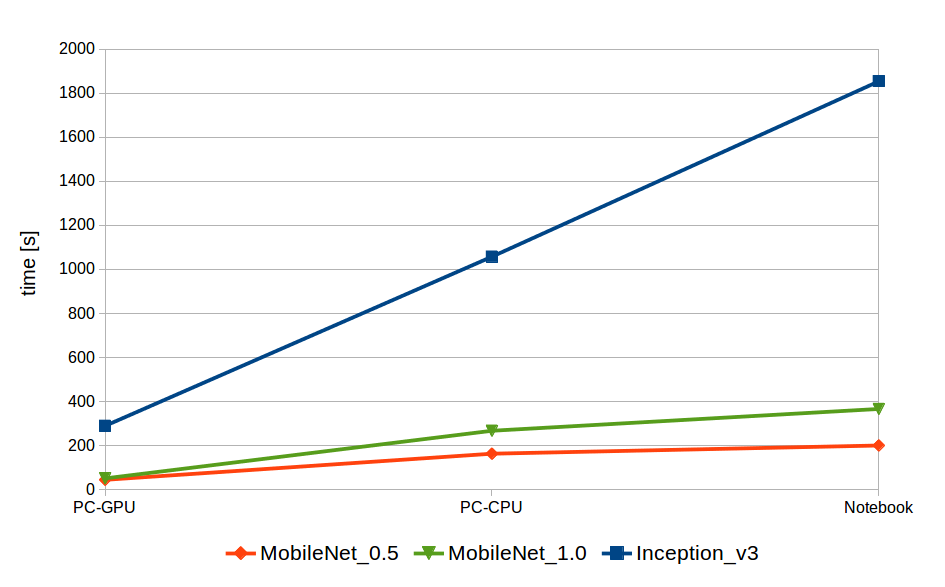
\includegraphics[width=0.9\textwidth]{includes/bottlenecks}
\caption[Total time creating bottlenecks]{Total time creating bottlenecks}
\label{fig:bottlenecks}
\end{figure}

Listing \ref{list:bottleneck_gpu} shows the workload of the GPU during calculating which can be showed by executing \textit{nvidia-smi -l 1}. It is working at 38\% capacity and uses about 3160 MiB memory. Whereas the CPU is only utilized at 110\% of the maximum 800\% because of four cores with hyper threading which can be seen in the top part of \figref{bottlenecksCPUUsage}. The bottom part of this figure shows about 470\% workload if calculating everything with desktop-CPU only.

\begin{minipage}{\linewidth}
\begin{lstlisting}[caption=Build and call of \textit{retrain}, label=list:bottleneck_gpu, language=bash]
	nvidia-smi -l 1
	| GPU  Name        Persistence-M| Bus-Id        Disp.A | Volatile Uncorr. ECC |
	| Fan  Temp  Perf  Pwr:Usage/Cap|         Memory-Usage | GPU-Util  Compute M. |
	|===============================+======================+======================|
	|   0  GeForce GTX 980     Off  | 00000000:01:00.0  On |                  N/A |
	|  1%   30C    P2    68W / 196W |   3873MiB /  4029MiB |     38%      Default |
	+-------------------------------+----------------------+----------------------+
	| Processes:                                                       GPU Memory |
	|  GPU       PID   Type   Process name                             Usage      |
	|=============================================================================|
	|    0      1065      G   /usr/lib/xorg/Xorg                           584MiB |
	|    0      1675      G   compiz                                        83MiB |
	|    0     12867      G   ...-token=A79FC92A8A549F181FB5DBE83D71EFC2    31MiB |
	|    0     26527      C   python                                      3159MiB |
\end{lstlisting}
\end{minipage}

\begin{figure}[htbp]
\centering
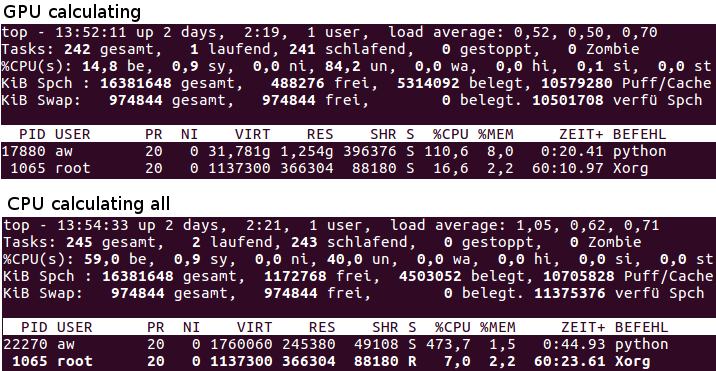
\includegraphics[width=0.7\textwidth]{includes/bottlenecksCPUUsage}
\caption[CPU usage creating bottlenecks]{CPU usage creating bottlenecks - Top: GPU - Bottom: CPU only}
\label{fig:bottlenecksCPUUsage}
\end{figure}

Once finished with creating the bottleneck values, training of the final layer begins. Each step random images of the training set will be fed into the final layer to get prediction. Those predictions are now used to update the final layer weigts through the back-propagation process. The script outputs the \textit{train accuracy}, \textit{cross entropy} and the \textit{validation accuracy} each 10th step as can be seen on \listref{training_hist}, which is a shortened output. At the end a final test evaluation with the testing image set is run which results in the \textit{final test accuracy}. Furthermore some time measurings are printed out. \citep{TensorFlowRetrain2017}

\begin{minipage}{\linewidth}
\begin{lstlisting}[caption=Output of \textit{retrain.py}, label=list:training_hist, language=bash]
	INFO:tensorflow:2018-01-23 18:49:46.730940: Step 0: Train accuracy = 34.0%
	INFO:tensorflow:2018-01-23 18:49:46.731069: Step 0: Cross entropy = 4.808121
	INFO:tensorflow:2018-01-23 18:49:46.839474: Step 0: Validation accuracy = 4.0% 
	INFO:tensorflow:2018-01-23 18:49:47.309740: Step 10: Train accuracy = 27.0%
	INFO:tensorflow:2018-01-23 18:49:47.309843: Step 10: Cross entropy = 4.646721
	INFO:tensorflow:2018-01-23 18:49:47.356538: Step 10: Validation accuracy = 15.0%
	INFO:tensorflow:2018-01-23 18:49:47.828190: Step 20: Train accuracy = 50.0%
	INFO:tensorflow:2018-01-23 18:49:47.828293: Step 20: Cross entropy = 4.465392
	INFO:tensorflow:2018-01-23 18:49:47.875599: Step 20: Validation accuracy = 32.0%
	### shortened ###
	INFO:tensorflow:2018-01-23 18:53:15.319134: Step 3990: Train accuracy = 91.0%
	INFO:tensorflow:2018-01-23 18:53:15.319235: Step 3990: Cross entropy = 0.282067
	INFO:tensorflow:2018-01-23 18:53:15.369910: Step 3990: Validation accuracy = 89.0%
	INFO:tensorflow:2018-01-23 18:53:15.796850: Step 3999: Train accuracy = 96.0%
	INFO:tensorflow:2018-01-23 18:53:15.796950: Step 3999: Cross entropy = 0.204091
	INFO:tensorflow:2018-01-23 18:53:15.844287: Step 3999: Validation accuracy = 89.0% 
	INFO:tensorflow:Final test accuracy = 91.0% (N=818)
	INFO:tensorflow:Froze 2 variables.
	Converted 2 variables to const ops.
	
	bottleneck time: 290.75745s
	Evaluation training time: 48.22647s
	Evaluation total time: 209.29127s
\end{lstlisting}
\end{minipage}

For explanation, \textit{train accuracy} shows the percentage of correctly labeled images in the current training batch. The \textit{validation accuracy} is also the percentage of correctly-labeled images but now on random images from the validation set. \textit{Cross entropy} is a loss function that indicates how well the learning process is progressing. \citep{TensorFlowRetrain2017}\\

If during training the error "Label xxx has no images in the category validation" occur, renaming this label names solves this issue because another hash will be calculated and the separation of the sets changes. \\

If using both, python and bazel execution methods the same version of TensorFlow has to be choosen, otherwise compatibility issues can occur! Especially the bazel one which is by default the newest version because of the master branch of github. \\


During the retrain process the outputted accuracies, cross entropy and some more data are written to the summaries directory and can be visualized with TensorBoard which is automatically installed with TensorFlow. To start it execute command in \listref{tensorboard}.

\begin{lstlisting}[caption=Build and call of \textit{retrain}, label=list:tensorboard, language=bash]
	tensorboard --logdir ${RETRAIN_PATH}/training_summaries/${ARCHITECTURE}_${TRAINING_STEPS}/ &
\end{lstlisting}

To validate the retrained model, see \subsecref{Output Tests and Validation}. \\

Now, also the graph of the model can be visualized in TensorBoard.
The retrained graph of the MobileNet model is depicted in \figref{graphMobilenet050-700} including the training nodes. In the appendix under \subsecref{} is a more detailed one with all convolutional layer and under \subsecref{} the view on the depthwise convolution containing its depthwise and pointwise convolutional layers as described in \subsecref{Common Models in Deep Learning Applications}. \\
The whole retrained graph of the MobileNet model is depicted in the appendix under \subsecref{}. Furthermore, under \subsecref{} a detailed view on a mixed_layer and under \subsecref{} it's specific operations within a convolutional layer. \\

\begin{figure}[htbp]
\centering
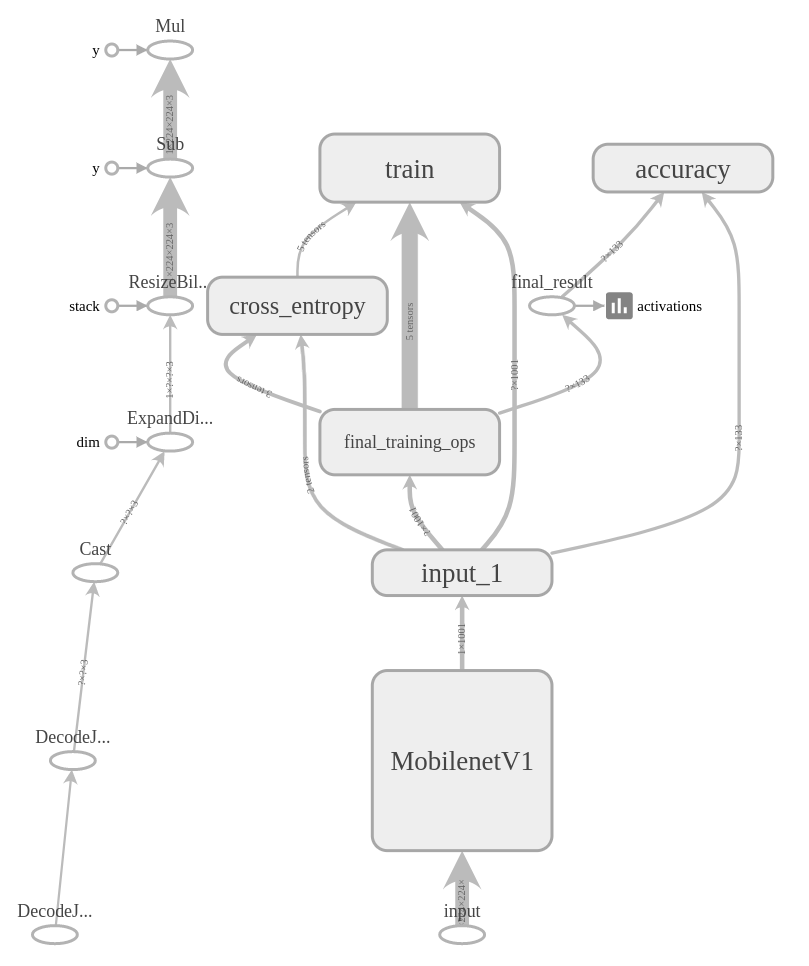
\includegraphics[height=10cm]{includes/graphMobilenet050-700}
\caption[MobileNet retrained graph]{MobileNet retrained graph}
\label{fig:graphMobilenet050-700}
\end{figure}



Playing around with the parameters \textit{how_many_training_steps} and \textit{learning_rate} can improve accuracy. To measure the performance of the network, the validation accuracy is a well indicator because these images aren't used for training. Even better to check the performance of the classification task is the evaluation test at the end of the retraining process, because those images are entirely unknown to the model.

"If the train accuracy is high but the validation accuracy remains low, that means the network is overfitting and memorizing particular features in the training images that aren't helpful more generally." \citep{TensorFlowRetrain2017} \\

In \figref{inception5000LR} the differences of retraining the InceptionV3 model with 5000 training steps and different learning rates is shown. For MobileNets it looks basically similar. 

\begin{figure}[htbp]
\centering
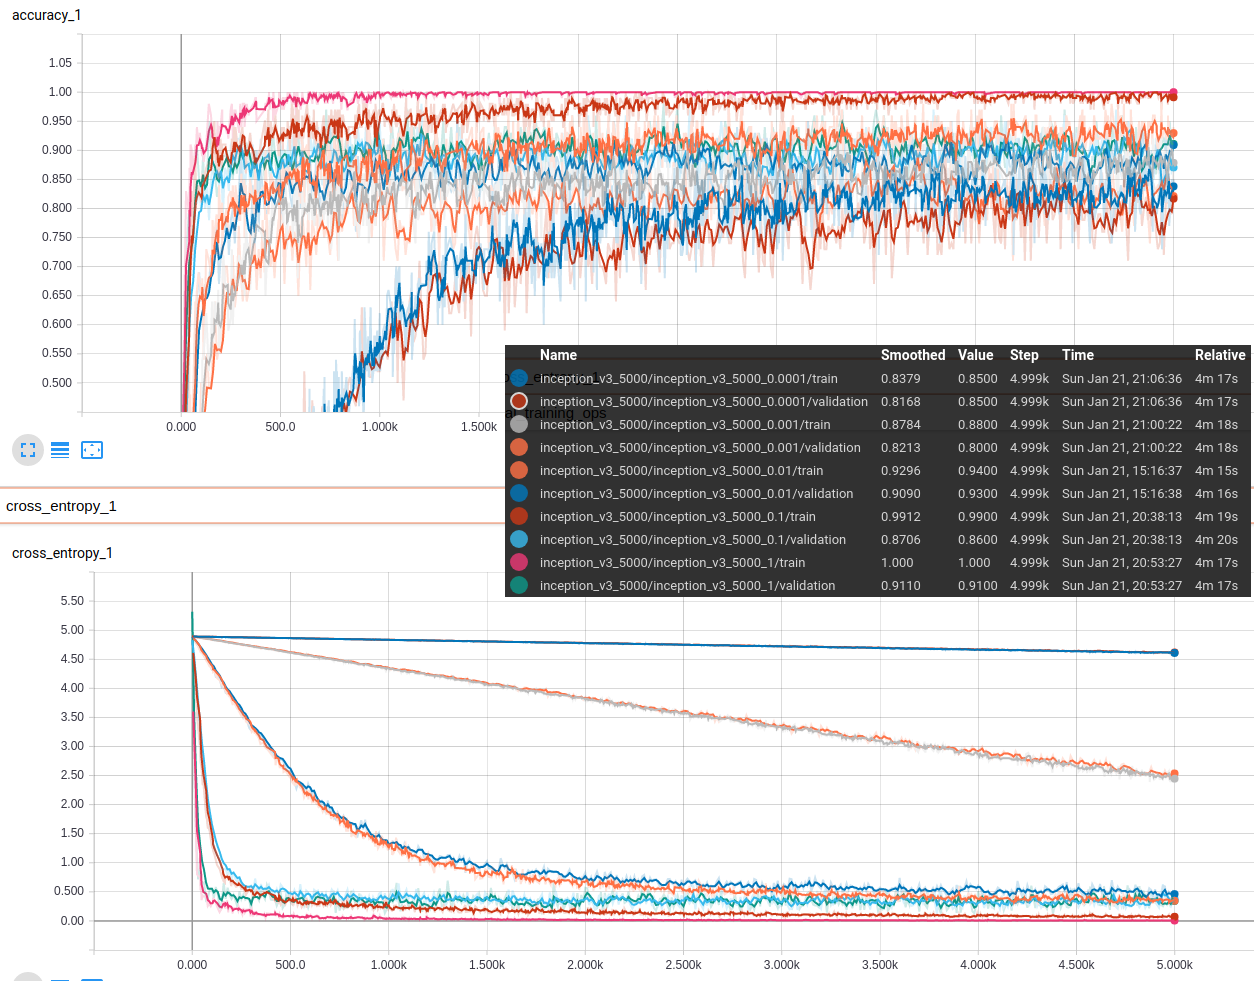
\includegraphics[width=0.95\textwidth]{includes/inception5000LR}
\caption[InceptionV3 with 5000 training steps and different learning rates]{InceptionV3 with 5000 training steps and different learning rates}
\label{fig:inception5000LR}
\end{figure}

The best values for the MobileNet0.5 model are 700 training steps and a learning rate of 0.007 (see result in \figref{MobileNet05-700res}).

For the MobileNet1.0 model it was hard to find really well values. So the best here are 500 training steps and a learning rate of 0.01 (see result in \figref{MobileNet10-500res}).

The final Inception model was retrained with 4000 training steps and a learning rate of 0.03 (see result in \figref{inception4000res}).

\begin{figure}[htbp]
\centering
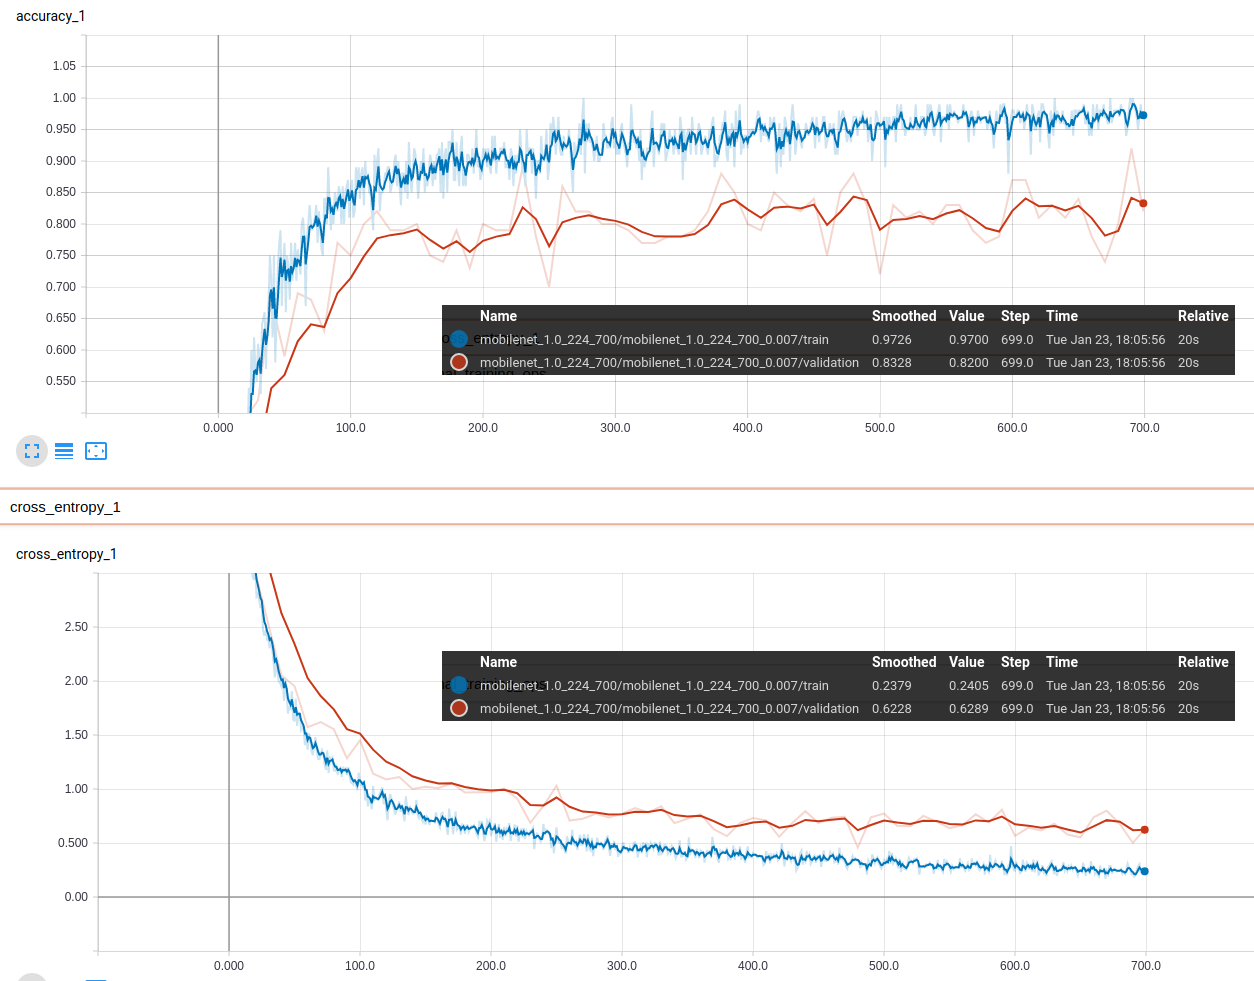
\includegraphics[width=0.95\textwidth]{includes/MobileNet05-700res}
\caption[MobileNet0.5 with 700 training steps and a learning rate of 0.007]{MobileNet0.5 with 700 training steps and a learning rate of 0.007}
\label{fig:MobileNet05-700res}
\end{figure}

\begin{figure}[htbp]
\centering
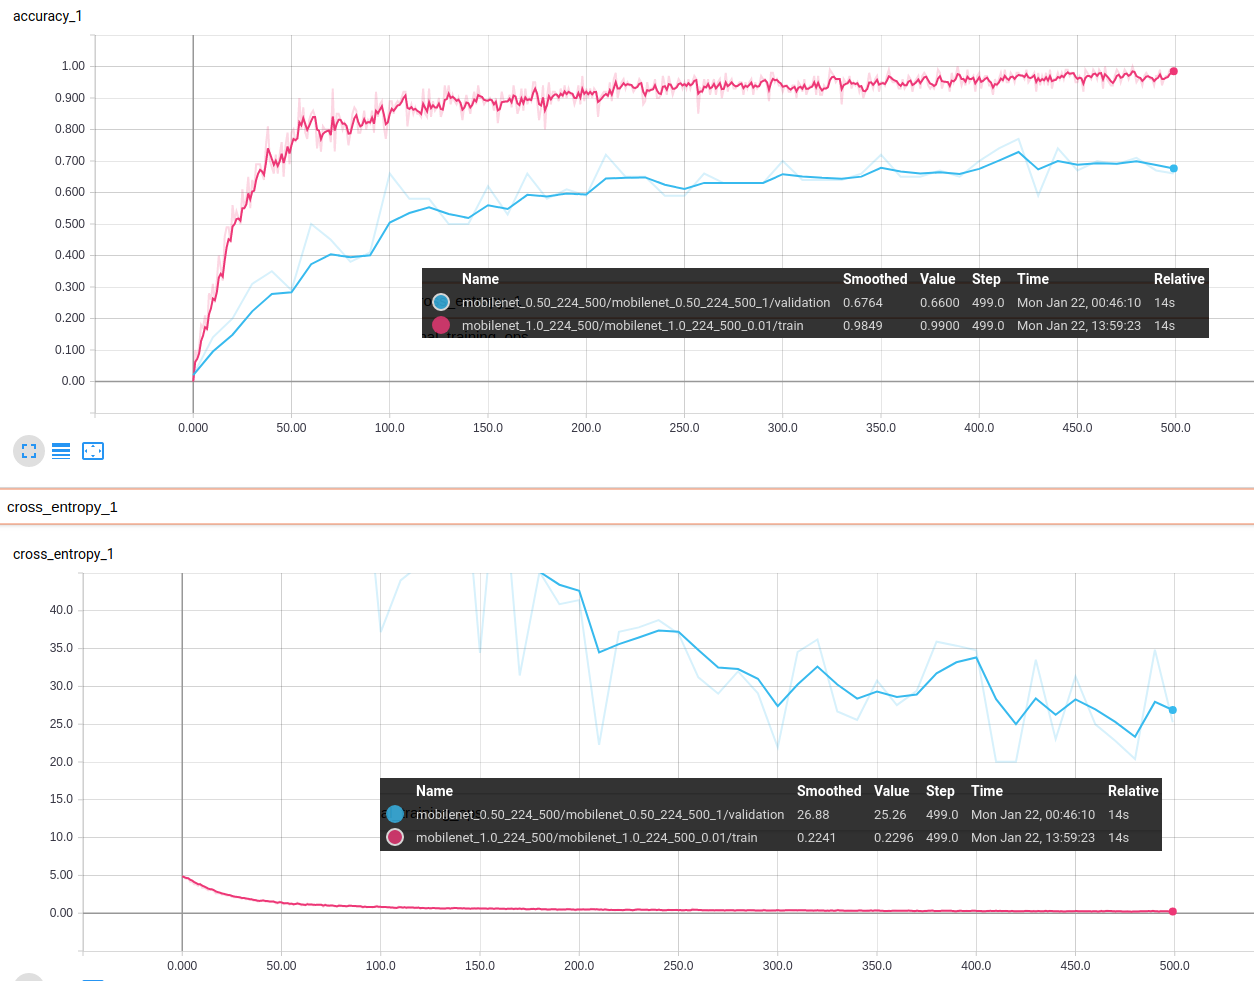
\includegraphics[width=0.95\textwidth]{includes/MobileNet10-500res}
\caption[MobileNet1.0 with 500 training steps and a learning rate of 0.01]{MobileNet1.0 with 500 training steps and a learning rate of 0.01}
\label{fig:MobileNet10-500res}
\end{figure}

\begin{figure}[htbp]
\centering
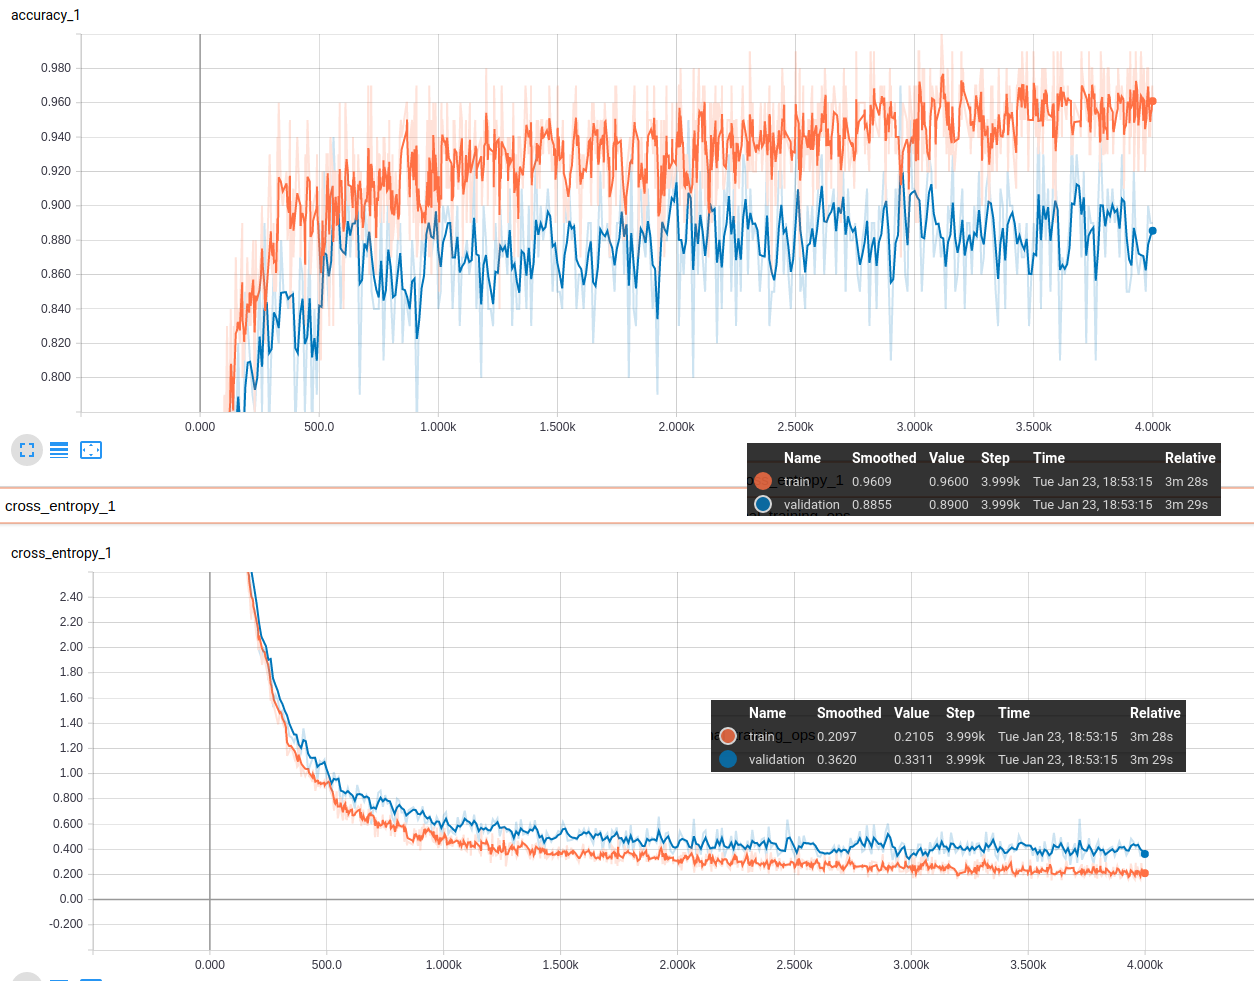
\includegraphics[width=0.95\textwidth]{includes/inception4000res}
\caption[InceptionV3 with 4000 training steps and a learning rates of 0.03]{InceptionV3 with 4000 training steps and a learning rates of 0.03}
\label{fig:inception4000res}
\end{figure}

ODER ALLES IN EINEM GRAPH \figref{AllRes} ODER ALLES IN ANHANG?!??! BZW das sollte in Evaluierung oder?!?

\begin{figure}[htbp]
\centering
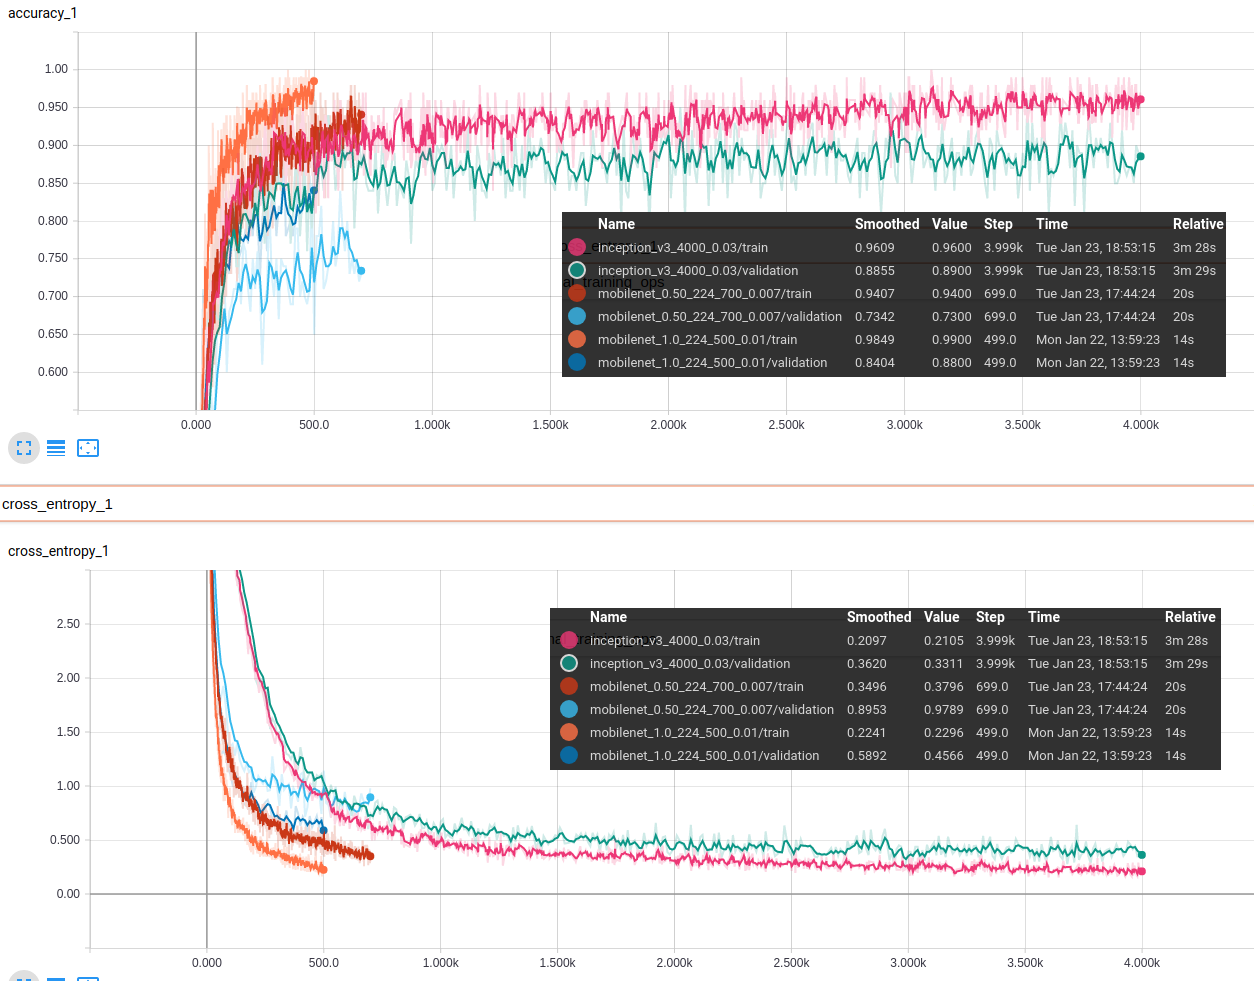
\includegraphics[width=0.95\textwidth]{includes/AllRes}
\caption[Diagram with best parameters for each model]{Diagram with best parameters for each model}
\label{fig:AllRes}
\end{figure}



As result of the retraining process the model is saved in the predefined file. So theoretically the models are now ready to use for inference. \\



However, to use the model in the mobile app, the DecodeJpeg Operation has to be stripped from the retrained model, because the Inference Interface of TensorFlow Mobile currently doesn't support it. This could be done by the \textit{strip_unused.py}-script of the official tensorflow github repository. \\

Nevertheless it is recommend to optimize the pretrained graph for mobile inference to achieve the best tradeoff between accuracy, latency, size and performance. There are several ways and different options to do the optimization. \\

The first one, which will be called in following as '\textit{opt1}', is only to run the \textit{optimize_for_inference}-script of the official tensorflow github repository. The corresponing call is shown in \listref{optimize_graph}.
This script removes all nodes that aren't needed anymore like all training operations, strips unused parts, removes debug informations, folding batch normalization ops into the pre-calculated weights and fusing common operations into unified versions.
 
\begin{minipage}{\linewidth}
\begin{lstlisting}[caption=Call of \textit{optimize_for_inference.py}, label=list:optimize_graph, language=bash]
	python -m tensorflow.python.tools.optimize_for_inference \
	  --input=${RETRAIN_PATH}/graphs/${ARCHITECTURE}_${TRAINING_STEPS}/retrained_dog_graph_${ARCHITECTURE}_${TRAINING_STEPS}_${LEARNING_RATE}.pb \
	  --output=${RETRAIN_PATH}/graphs/${ARCHITECTURE}_${TRAINING_STEPS}/opt1_retrained_dog_graph_${ARCHITECTURE}_${TRAINING_STEPS}_${LEARNING_RATE}.pb \
	  --input_names=${INPUT_LAYER} \
	  --output_names="final_result"
\end{lstlisting}
\end{minipage}

The next attempt is to use the already optimized graph of \textit{opt1} and additionally quantizes the graph by rounding the weights. Using the script of tensorflow-for-poets-2-tutorial and calling it as shown in \listref{quantize_graph}). This will make the model compressible, which will reduce the model size significantly, thus every mobile app compresses the package before distribution.

\begin{minipage}{\linewidth}
\begin{lstlisting}[caption=Call of \textit{quantize_graph.py}, label=list:quantize_graph, language=bash]
	python -m scripts.quantize_graph \
	  --input=${RETRAIN_PATH}/graphs/${ARCHITECTURE}_${TRAINING_STEPS}/opt1_retrained_dog_graph_${ARCHITECTURE}_${TRAINING_STEPS}_${LEARNING_RATE}.pb \
	  --output=${RETRAIN_PATH}/graphs/${ARCHITECTURE}_${TRAINING_STEPS}/opt2_retrained_dog_graph_${ARCHITECTURE}_${TRAINING_STEPS}_${LEARNING_RATE}.pb \
	  --output_node_names=final_result \
	  --mode=weights_rounded
\end{lstlisting}
\end{minipage}

To compare the improvement, use the gzip command in \listref{gzip} on the model of \textit{opt1} and also on this new one. 

\begin{minipage}{\linewidth}
\begin{lstlisting}[caption=Call of gzip, label=list:gzip, language=bash]
	gzip -c ${RETRAIN_PATH}/graphs/${ARCHITECTURE}_${TRAINING_STEPS}/retrained_dog_graph_${ARCHITECTURE}_${TRAINING_STEPS}_${LEARNING_RATE}.pb > ${RETRAIN_PATH}/graphs/${ARCHITECTURE}_${TRAINING_STEPS}/retrained_dog_graph_${ARCHITECTURE}_${TRAINING_STEPS}_${LEARNING_RATE}.pb.gz

	gzip -l ${RETRAIN_PATH}/graphs/${ARCHITECTURE}_${TRAINING_STEPS}/retrained_dog_graph_${ARCHITECTURE}_${TRAINING_STEPS}_${LEARNING_RATE}.pb.gz
\end{lstlisting}
\end{minipage}

The detailed result starting with the \textit{opt1} output and then ending with the \textit{opt2} output is shown in \listref{gzip_res}. So the \textit{opt2} model is 65,4\% lower in size and that's independent of the model used. 

As example with the InceptionV3 model the size is dropped from about 88 MB to only 24 MB which is a great improvement.

\begin{minipage}{\linewidth}
\begin{lstlisting}[caption=Output of gzip, label=list:gzip_res, language=bash]
	compressed	uncompressed	ratio	uncompressed_name
	81839945	88222145	7,20%	/home/aw/MobileInceptionRetrained/graphs/inception_v3_4000/opt1_retrained_dog_graph_inception_v3_4000_0.03.pb

	compressed	uncompressed	ratio	uncompressed_name
	24164803	88224397	72,60%	/home/aw/MobileInceptionRetrained/graphs/inception_v3_4000/opt2_retrained_dog_graph_inception_v3_4000_0.03.pb
\end{lstlisting}
\end{minipage}


These first two ways of optimization are described in the tensorflow-for-poets-2-tutorial. 

The next two attempts are using \textit{transform_graph} of the official tensorflow github repository. Unfortunately there exists none python version of that tool, so it has to be built with bazel first. 

The tool \textit{transform_graph} has an parameter, called \textit{tranforms}, which defines all operations to be executed. Calling the commands in \listref{transform_graph_opt3} strips all unused nodes and folding batch normalization ops, so very similar to \textit{opt1}. This will be \textit{opt3} in the following content.

\begin{minipage}{\linewidth}
\begin{lstlisting}[caption=Build and call of \textit{transform_graph}, label=list:transform_graph_opt3, language=bash]
	bazel build tensorflow/tools/graph_transforms:transform_graph && \
	bazel-bin/tensorflow/tools/graph_transforms/transform_graph \
	--in_graph=${RETRAIN_PATH}/graphs/${ARCHITECTURE}_${TRAINING_STEPS}/retrained_dog_graph_${ARCHITECTURE}_${TRAINING_STEPS}_${LEARNING_RATE}.pb \
	--out_graph=${RETRAIN_PATH}/graphs/${ARCHITECTURE}_${TRAINING_STEPS}/opt3_retrained_dog_graph_${ARCHITECTURE}_${TRAINING_STEPS}_${LEARNING_RATE}.pb \
	--inputs=${INPUT_LAYER} \
	--outputs='final_result:0' \
	--transforms='
		strip_unused_nodes(type=float, shape="1,${INPUT_SIZE},${INPUT_SIZE},3")
		remove_nodes(op=Identity, op=CheckNumerics)
		fold_old_batch_norms'
\end{lstlisting}
\end{minipage}

With \textit{opt4} the command in \listref{transform_graph_opt4} has been extended by \textit{fold_old_batch_norms}, \textit{round_weights} and \textit{sort_by_execution_order}. Thus this one also rounds the weights, it is also compressible, which is similar to the \textit{opt2} one. 

\begin{minipage}{\linewidth}
\begin{lstlisting}[caption=Build and call of \textit{transform_graph}, label=list:transform_graph_opt4, language=bash]
	bazel build tensorflow/tools/graph_transforms:transform_graph && \
	bazel-bin/tensorflow/tools/graph_transforms/transform_graph \
	--in_graph=${RETRAIN_PATH}/graphs/${ARCHITECTURE}_${TRAINING_STEPS}/retrained_dog_graph_${ARCHITECTURE}_${TRAINING_STEPS}_${LEARNING_RATE}.pb \
	--out_graph=${RETRAIN_PATH}/graphs/${ARCHITECTURE}_${TRAINING_STEPS}/opt4_retrained_dog_graph_${ARCHITECTURE}_${TRAINING_STEPS}_${LEARNING_RATE}.pb \
	--inputs=${INPUT_LAYER} \
	--outputs=final_result:0 \
	--transforms=' 
		strip_unused_nodes(type=float, shape="1,${INPUT_SIZE},${INPUT_SIZE},3")
		remove_nodes(op=Identity, op=CheckNumerics) 
		fold_batch_norms 
		fold_old_batch_norms 
		round_weights(num_steps=256)
		sort_by_execution_order'
\end{lstlisting}
\end{minipage}


There are several helper tools, two of them are definitely worth to introduce here right now. \\

The first one, is the \textit{graph_pb2tb.py}-script, again from the tensorflow-for-poets-tutorial. It generates a summary file, similar than during retraining process, except that only the data of the graph is stored for visualization with TensorBoard. So after optimizing the graph and calling the command of \listref{graph_pb2tb} the graph of the MobileNet model should look like depicted in \figref{MobileNetGraphOpt4} which is completely stripped of unused nodes as the training stuff and thus optimized for inference. The InceptionV3 model is in the appendix under \subsecref{Optimized InceptionV3 model}. \\

\begin{minipage}{\linewidth}
\begin{lstlisting}[caption=Call of \textit{graph_pb2tb.py}, label=list:graph_pb2tb, language=bash]
	python -m scripts.graph_pb2tb ${RETRAIN_PATH}/training_summaries/${ARCHITECTURE}_${TRAINING_STEPS}/${ARCHITECTURE}_${TRAINING_STEPS}_${LEARNING_RATE}/retrained \
	  ${RETRAIN_PATH}/graphs/${ARCHITECTURE}_${TRAINING_STEPS}/retrained_dog_graph_${ARCHITECTURE}_${TRAINING_STEPS}_${LEARNING_RATE}.pb 
\end{lstlisting}
\end{minipage}

\begin{figure}[htbp]
\centering
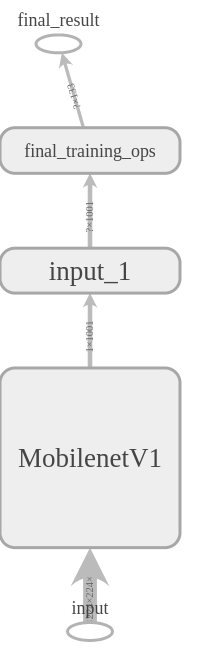
\includegraphics[height=7cm]{includes/graphMobilenet050-700Opt4}
\caption[Optimized graph of a MobileNet model]{Optimized graph of a MobileNet model}
\label{fig:MobileNetGraphOpt4}
\end{figure}


The other tool is \textit{summarize_graph} of the official tensorflow github repository, which has to be built by bazel. After building and calling command of \listref{summarize_graph} a short summary of the model is printed out which includes useful information like the shape, the name of input and output layers or quantity of constants. An example with the optimized retrained InceptionV3 model is shown in \listref{summarize_graph_out}.

\begin{minipage}{\linewidth}
\begin{lstlisting}[caption=Build and call of \textit{summarize_graph}, label=list:summarize_graph, language=bash]
	bazel build tensorflow/tools/graph_transforms:summarize_graph && \
	bazel-bin/tensorflow/tools/graph_transforms/summarize_graph \
		--in_graph=${RETRAIN_PATH}/graphs/${ARCHITECTURE}_${TRAINING_STEPS}/retrained_dog_graph_${ARCHITECTURE}_${TRAINING_STEPS}_${LEARNING_RATE}.pb
\end{lstlisting}
\end{minipage}

\begin{minipage}{\linewidth}
\begin{lstlisting}[caption=Output of \textit{summarize_graph} on a retrained and optimized InceptionV3 model, label=list:summarize_graph_out, language=bash]
	Found 1 possible inputs: (name=Mul, type=float(1), shape=[1,299,299,3]) 
	No variables spotted.
	Found 1 possible outputs: (name=final_result, op=Softmax) 
	Found 22040882 (22.04M) const parameters, 0 (0) variable parameters, and 0 control_edges
	Op types used: 202 Const, 94 BiasAdd, 94 Conv2D, 94 Relu, 11 Concat, 9 AvgPool, 5 MaxPool, 1 Add, 1 MatMul, 1 	Placeholder, 1 PlaceholderWithDefault, 1 Reshape, 1 Softmax
\end{lstlisting}
\end{minipage}



	\mysubsection{Output Tests and Validation}
In order to test and validate the output of the model regardless of whether the pretrained, retrained or optimized one is used the python script named \textit{label\_image}.py of the 'tensorflow-for-poets'-tutorial was applied. Three variables has to be defined differently which is shown at the beginning of \listref{label_image}. Depending which model is used for labeling an image, the first or second section must be applied.

\begin{minipage}{\linewidth}
\begin{lstlisting}[caption=Call of \textit{label\_image.py}, label=list:label_image, language=bash]
	#for InceptionV3 models	use:
	INPUT_SIZE=299			#size of input layer
	INPUT_LAYER=Mul		#name of input layer
	OUTPUT_LAYER=softmax	#name of output layer (only for pretrained model otherwise 'final_result' or as defined in retrain-script)
	
	#for MobileNet models use:
	INPUT_SIZE=224			#size of input layer
	INPUT_LAYER=input	 	#name of input layer
	OUTPUT_LAYER=MobilenetV1/Predictions/Reshape_1	#name of output layer (only for pretrained model otherwise 'final_result' or as defined in retrain-script)

	python -m scripts.label_image \
	--graph=${HOME}/retrained_graph.pb \
	--labels=${HOME}/retrained_labels.txt \
	--output_layer=final_result \
	--input_layer=${INPUT_LAYER} \
	--image=${HOME}/dl/label_image_pics/Affenpinscher_00001.jpg \
	--input_width=${INPUT_SIZE} \
	--input_height=${INPUT_SIZE}
\end{lstlisting}
\end{minipage}

The corresponding command based on Bazel is shown in \listref{label_image} where again the three variables need to be specified. The call itself is fundamentally the same. However, the executable binary has to be built before which is shown in \listref{blabel_image}.

\begin{minipage}{\linewidth}
\begin{lstlisting}[caption=Build and call of \textit{label\_image}, label=list:blabel_image, language=bash]
	bazel build tensorflow/examples/label_image:label_image && \
	bazel-bin/tensorflow/examples/label_image/label_image \
		--graph=${HOME}/retrained_graph.pb \
		--labels=${HOME}/retrained_labels.txt \
		--output_layer=final_result \
		--input_layer=${INPUT_LAYER} \
		--image=${HOME}/dl/label_image_pics/Affenpinscher_00001.jpg \
		--input_width=${INPUT_SIZE} \
		--input_height=${INPUT_SIZE}
\end{lstlisting}
\end{minipage}

If retraining of the model was conducted successfully, the output of \textit{label\_image} consists of five labels containing the highest values and corresponding accuracy which are returned by the model (refer to \listref{label_imageOutput}).

\begin{minipage}{\linewidth}
\begin{lstlisting}[caption=Output of \textit{label\_image.py}, label=list:label_imageOutput, language=bash]
	Evaluation time (1-image): 0.350s
	
	001 affenpinscher 0.9940035
	038 brussels griffon 0.002003342
	042 cairn terrier 0.0008437461
	100 lowchen 0.00018292216
	099 lhasa apso 0.00012668292
\end{lstlisting}
\end{minipage}




	\mysubsection{Implementation of an native Android App} 
This subchapter describes the processing of the camera input stream and classifying the particular images. Because of the vast extent of the application, the focus lies on the explanation of how the app works and on its important implementation parts. \\

When clicking on the icon of the app, a camera view showing results in the bottom part is loaded. In the background, the ClassifierActivity is set as the launcher activity in the AndroidManifest.xml which is a file containing all configuration settings for the app. When an activity is loaded for the first time, the onCreate method is invoked. Because the ClassifierActivity extends the CameraActivity the onCreate method of the CameraActivity is executed and loads the layout activity_camera.xml consisting of a container and a result field. Next, the setFragment method of the class CameraActivity is invoked if permission for the camera is given. This causes the replacement of the container with the adapted fragment according to the actual size and orientation of the screen. When the size is set, the method onPreviewSizeChosen is invoked where a TensorFlowImageClassifier is instantiated with following input parameters: MODEL_FILE, LABEL_FILE, INPUT_SIZE, IMAGE_MEAN, IMAGE_STD, INPUT_NAME, OUTPUT_NAME. Details about the classification itself follow later in the section.\\

When the fragment was replaced by the CameraActivity, an instance of the class CameraFragment was created. Next, the method onViewCreated of the class CameraFragment is called and a texture view is created. The latter class is part of the Android API and used for frame capturing from an image stream as OPENGL ES texture. Thereby, the most recent image is stored within a texture object. This object is observed by a listener which invokes the method onSurfaceTextureAvailable when the texture object is available. Within this method the camera is opened by the method openCamera(width, height) given the width and height of the camera preview \citep{AndroidDevelopers}. First, the method openCamera sets the camera parameters within setUpCameraOutputs e.g. sensorOrientation, previewSize, cameraId etc. In order to classifiy a given OPENGL ES texture, the coordinate column vectors of the texture must be transformed into the proper sampling location in the streamed texture. So, the matrix has to be prepared with the correct configuration which happens in the method configureTransform. The next important step is done by the camera manager which opens the camera by invoking the method openCamer(cameraId, stateCallback, backgroundHandler). The id represents the specific camera device whereas the stateCallback is necessary to manage the life circle of the camera device and to handle different states of the camera device. The backgroundHandler ensures that the classification is done in background mode. When the camera is opened, the camera preview is started by the method createCameraPreviewSession. Within this method the preview reader is initialized and set to read images from the ImageListener which observes whether an image is available. Therefore, an Imagelistener which was instantiated by the CameraActivity is transfered to the CameraFragment. \\

When an image is available the method onImageAvailable of the class ClassifierActivity is invoked. The image is read by the preview reader and stored in an object. First, the image is preprocessed meaning transfered into planes, stored as bytes, cropped and stored as a Bitmap which is an Android graphic. Google provides an Tensorlflow Mobile API to run tensors on a performance critical device such as mobile devices. To use this API, the dependency has to be added to the build.gradle file as shown in\listref{tensorflow_api}. 

\begin{lstlisting}[caption=Tensorflow API in build.gradle, label=list:tensorflow_api, language=java]
	allprojects {
  		repositories {
        	jcenter()
    	}
	}

	dependencies {
    	compile 'org.tensorflow:tensorflow-android:+'
	}
\end{lstlisting}

When including the API, Tensorflow's class Classifier can be used to classify images. Therefore, the TensorFlowImageClassifier which was initialized before invokes the method recognizeImage(croppedBitmap) on the preprocessed image. Within this method, the image data is transfered from int to float (refer to \listref{int_conversion}). Then, the previous initialized object of the TensorflowInferenceInterface calls the method feed to pass the float values to the input layer of the model. Afterwards, the inferenceInterface invokes the method run with the specified output layer in order to process the classification. Subsequently, the output data is fetched by calling fetch on the output layer which is depicted in \listref{classify_android}.

\begin{lstlisting}[caption=Classifying images by the inferenceInterface, label=list:classify_android, language=java]

    // Copy the input data into TensorFlow.
    Trace.beginSection("feed");
    inferenceInterface.feed(inputName, floatValues, 1, inputSize, inputSize, 3);
    Trace.endSection();

    // Run the inference call.
    Trace.beginSection("run");
    inferenceInterface.run(outputNames, logStats);
    Trace.endSection();

    // Copy the output Tensor back into the output array.
    Trace.beginSection("fetch");
    inferenceInterface.fetch(outputName, outputs);
    Trace.endSection();
\end{lstlisting}

Afterwards, the results are reordered according to the highest probability and returned to the result field for displaying the output.

	\mysubsection{Deployment and Validation} 
In order to get the model running in the application, a few things must be adapted. First, the model in the format of a .pb file and its retrained labels as a text file must be imported. Therefore, a assets folder was created where the model and labels were placed. Next, the path of the model and the labels file must be specified like pictured in \listref{include_model}.

\begin{lstlisting}[caption=Including the model in the mobile application, label=list:include_model, language=java]
    // Input shapes
    private static final int INPUT_SIZE = 224;
    private static final int IMAGE_MEAN = 128;
    private static final float IMAGE_STD = 128.0f;

    // Input Layer
    private static final String INPUT_NAME = "input";

    // Output Layer
    private static final String OUTPUT_NAME = "final_result";

    // Model Name from Assets
    private static final String MODEL_FILE = "file:///android_asset/				opt4_retrained_dog_graph_mobilenet_0.50_224_700_0.007.pb";


    // Label Name from Assets
    private static final String LABEL_FILE = "file:///android_asset/retrained_dog_labels_mobilenet_0.50_224_700_0.007.txt";

\end{lstlisting}

For MobileNet models the default settings are shown in the mentioned listing. Otherwise, if an InceptionV3 is used, the settings must be adapted like shown in \listref{include_inception}.

\begin{lstlisting}[caption=Setup for InceptionV3, label=list:include_inception, language=java]
    private static final int INPUT_SIZE = 299;
    private static final int IMAGE_MEAN = 128;
    private static final float IMAGE_STD = 128.0f;
    private static final String INPUT_NAME = "Mul:0";
    private static final String OUTPUT_NAME = "final_result";
\end{lstlisting}

The input size defines the size of the input layer of InceptionV3 which is 'Mul'. Whereas the input layer for MobileNet is specified as 'input'. The IMAGE_MEAN and IMAGE_STD values are needed for converting the image data from integer into float values. The conversion is shown in \listref{int_conversion}.

\begin{lstlisting}[caption=Conversion of image data integer to float, label=list:int_conversion, language=java]
	for (int i = 0; i < intValues.length; ++i) {
      final int val = intValues[i];
      floatValues[i * 3 + 0] = (((val >> 16) & 0xFF) - imageMean) / imageStd;
      floatValues[i * 3 + 1] = (((val >> 8) & 0xFF) - imageMean) / imageStd;
      floatValues[i * 3 + 2] = ((val & 0xFF) - imageMean) / imageStd;
    }
\end{lstlisting}

Futhermore, the output layer has to be specified. For MobileNet and InceptionV3, this was set to 'final_result'. \\

After setting up the application with appropriate values, the application can be built and run. If the application is running successfully and doesn't terminate, the settings are correct. If the result view contains results, everthing's working. If the results are below 0.1, the threshold in the class TensorflowImageClassifier has to be adapted. It's default setting is 0.01f which means only relevant results higher than 0.01 are shown in the result field. As a consequence, bad results given by the network aren't shown in general. In this case, we optimized the model again instead of lower the threshold. Just for the validation of a correct working app, the threshold was set to 0.001f.